\section{Sorting problem}

The sorting problem is a fundamental computational task that involves arranging a collection of elements in a specific order, typically ascending or descending. 
The input is an unsorted list or array, and the goal is to rearrange the elements such that they follow a predefined sequence based on some criteria.

\subsection{Quicksort}
Quicksort is a highly efficient divide-and-conquer sorting algorithm proposed by Hoare in 1962. 
It is widely used due to its practical performance and ability to sort in-place, meaning it requires only a small, constant amount of extra storage space. 
With proper tuning, Quicksort outperforms many other algorithms in practical applications.
\begin{enumerate}
    \item \textit{Divide}: select a pivot element from the array and partition the array into two subarrays:
        \begin{itemize}
            \item Elements in the lower subarray are less than or equal to the pivot.
            \item Elements in the upper subarray are greater than or equal to the pivot.
        \end{itemize}
    \item \textit{Conquer}: recursively apply quicksort to each of the two subarrays.
    \item \textit{Combine}: since the subarrays are already sorted, no additional work is needed to combine them.
\end{enumerate}
The key to quicksort's efficiency is the linear-time partitioning subroutine, which runs in $\mathcal{O}(n)$ time. 

Given an array $A[p\cdots q]$, the goal is to select a pivot element $x$ and rearrange the array so that all elements less than $x$ appear before it, and all elements greater than or equal to $x$ appear after it.
\begin{algorithm}[H]
    \caption{Quicksort}
    \begin{algorithmic}[1]
        \Function{partition}{$A,p,q$}
            \State $x=A[p]$
            \State $i=p$
            \For {$j=p+1$\textbf{ to }$q$}
                \If {$A[j]\leq x$}
                    \State {$i=i+1$}
                    \State \textbf{exchange }$A[i]\leftrightarrow A[j]$
                \EndIf
            \EndFor
            \State \textbf{exchange }$A[p]\leftrightarrow A[i]$
            \State \Return $i$
        \EndFunction
        \Statex
        \Procedure{quicksort}{$A,p,r$}
            \If {$p<r$}
                \State $q=$\Call{partition}{$A,p,r$}
                \State \Call{quicksort}{$A,p,q-1$}
                \State \Call{quicksort}{$A,q+1,r$}
            \EndIf
        \EndProcedure
    \end{algorithmic}
\end{algorithm}  

\paragraph*{Worst case complexity}
The worst case occurs when the pivot element always ends up at one of the ends of the array, resulting in highly unbalanced partitions. 
In this case, the recurrence relation for the running time is:
\[T(n) = T(0) + T(n - 1) + \Theta(n)\]
This leads to the worst-case time complexity of $\Theta(n^2)$.

\paragraph*{Best case complexity}
In the best case, the partitioning process splits the array into two even halves. 
The recurrence relation for the best case is:
\[T(n) = 2T\left(\dfrac{n}{2}\right) + \Theta(n)\]
Solving this recurrence gives a time complexity of $\Theta(n \log n)$, which is typical for efficient sorting algorithms.

\paragraph*{Average case complexity}
Even though the worst-case scenario yields $\Theta(n^2)$, quicksort's average-case time complexity is $\Theta(n \log n)$.
This happens because, on average, the pivot tends to split the array into reasonably balanced parts, making the overall performance efficient for large datasets.

\paragraph*{Unbalanced case Complexity}
If the partitioning process always splits the array in a highly unbalanced way, such as 10\% and 90\% split, the recurrence is:
\[T(n)=T\left(\dfrac{1}{10}n\right)+T\left(\dfrac{9}{10}n\right)+\Theta(n)\]
Even in such cases, the overall time complexity remains $\Theta(n\lg n)$, although the constant factors may differ. 

In practice, specialized partitioning strategies are used to efficiently handle cases where there are duplicate elements in the input array.
The performance of quicksort is highly dependent on the choice of the pivot. 
Common strategies include selecting the first element, the last element, or the median-of-three (choosing the median of the first, middle, and last elements).

\subsection{Randomized quicksort}
Randomized quicksort is an enhanced version of the classic quicksort algorithm. 
It improves performance by ensuring that the pivot is selected randomly, thus minimizing the likelihood of worst-case behavior. 
This approach ensures that the running time is not dependent on the input's structure.
The running time is independent of the input's initial order, avoiding worst-case scenarios caused by already sorted or reverse-ordered data.

Suppose we alternate between lucky and unlucky partitioning scenarios:
\begin{itemize}
    \item \textit{Lucky scenario}: the pivot divides the array evenly, making recursive calls on approximately half the array each time: 
        \[L(n) = 2U\left(\dfrac{n}{2}\right) + Q(n)\]
    \item \textit{Unlucky scenario}: the pivot divides the array in a highly unbalanced way, for example, making a recursive call on almost the entire array: 
        \[U(n) = L(n - 1) + Q(n)\]
\end{itemize}
Solving this system gives us:
\[L(n) = 2\left(L\left(\dfrac{n}{2}-1\right) + Q\left(\dfrac{n}{2}\right)\right) + Q(n)\]
This simplifies to:
\[L(n)= Q(n \log n)\]
Thus, the randomized pivot selection helps ensure that the algorithm performs efficiently in expectation, typically resulting in a time complexity of $\mathcal{O}(n \log n)$. 

\paragraph*{Analysis}
Let $T(n)$ be the random variable for the running time of randomized Quicksort on an input of size $n$, assuming that the random numbers are independent.
For $k=0,1,\dots,n-1$, define an indicator random variable $X_k$, where:
\[X_k=\begin{cases}
    1 \qquad \text{if PARTITION generates a k : n-k-1 split} \\
    0 \qquad \text{otherwise}
\end{cases}\]
The expected value of $X_k$ is: 
\[\mathbb{E}[X_k] = \Pr{X_k = 1} = \dfrac{1}{n}\]
This is because all splits are equally likely, assuming the elements are distinct. 
Therefore, the expected running time of the algorithm can be written as:
\[\mathbb{E}[T(n)] = \mathbb{E} \left[ \sum_{k=0}^{n-1} X_k \left( T(k) + T(n - k - 1) + \Theta(n) \right) \right]\]
Breaking this down:
\[\mathbb{E}[T(n)] =\frac{1}{n} \sum_{k=0}^{n-1} \mathbb{E}[T(k)] + \frac{1}{n} \sum_{k=0}^{n-1} \mathbb{E}[T(n - k - 1)] + \frac{1}{n} \sum_{k=0}^{n-1} \Theta(n)\]
This simplifies to:
\[\mathbb{E}[T(n)] =\frac{2}{n} \sum_{k=1}^{n} \mathbb{E}[T(k)] + \Theta(n)\]


In this case we have: 
\begin{align*}
     \\
            &= \sum_{k=0}^{n-1} \mathbb{E} \left[ X_k \left( T(k) + T(n - k - 1) + \Theta(n) \right) \right] \\
            &= \sum_{k=0}^{n-1} \mathbb{E}[X_k] \cdot E \left[ T(k) + T(n - k - 1) + \Theta(n) \right] \\
            &= 
            &= 
\end{align*}
For large enough $n$, where $n \geq 2$, we find that:
\[\mathbb{E}[T(n)]\leq \frac{2}{n} \sum_{k=1}^{n} ak\log k + \Theta(n)\leq an\log n\]
Thus, for a sufficiently large constant $a$, the $\Theta(n)$ term is dominated, leading to an overall time complexity of $\mathcal{O}(n\log n)$. 

Randomized quicksort is generally more than twice as fast as merge sort in practice.
Quicksort's performance can be improved significantly with careful code tuning and optimized implementations.
It behaves well with caching and virtual memory, making it suitable for use in systems with large datasets or hierarchical memory structures.

\subsection{Comparison sort analysis}
All the sorting algorithms discussed so far belong to the class of comparison sorts.
In these algorithms, sorting is achieved by performing pairwise comparisons between elements to determine their relative order.
The best worst-case time complexity we have seen for these comparison-based sorting algorithms is $\mathcal{O}(n\log n)$. 

To understand why $\mathcal{O}(n\log n)$ is the best achievable worst-case performance for comparison sorts, we can model sorting algorithms using decision trees. 

Consider sorting an array $\left\langle a_1,a_2,\dots,a_n\right\rangle$. 
We represent each comparison made by the sorting algorithm as a node in a decision tree.
Each internal node in this tree corresponds to a comparison between two elements $a_i$ and $a_j$ from the array. 
The tree has the following properties:
\begin{itemize}
    \item Each internal node is labeled with a pair $i$,$j$ (indices of elements being compared).
    \item The left child represents the path taken if $a_i \leq a_j$, while the right child represents the path if $a_i > a_j$. 
\end{itemize}
Each leaf node in the tree represents one of the possible final sorted orders (permutations) of the array. 
The entire tree represents all possible sequences of comparisons that can occur for different input arrays of size $n$. 
\begin{example}
    Consider sorting the array $\left\langle 9,4,6\right\rangle$. 
    The corresponding decision tree might look like the following: 
    \begin{figure}[H]
        \centering
        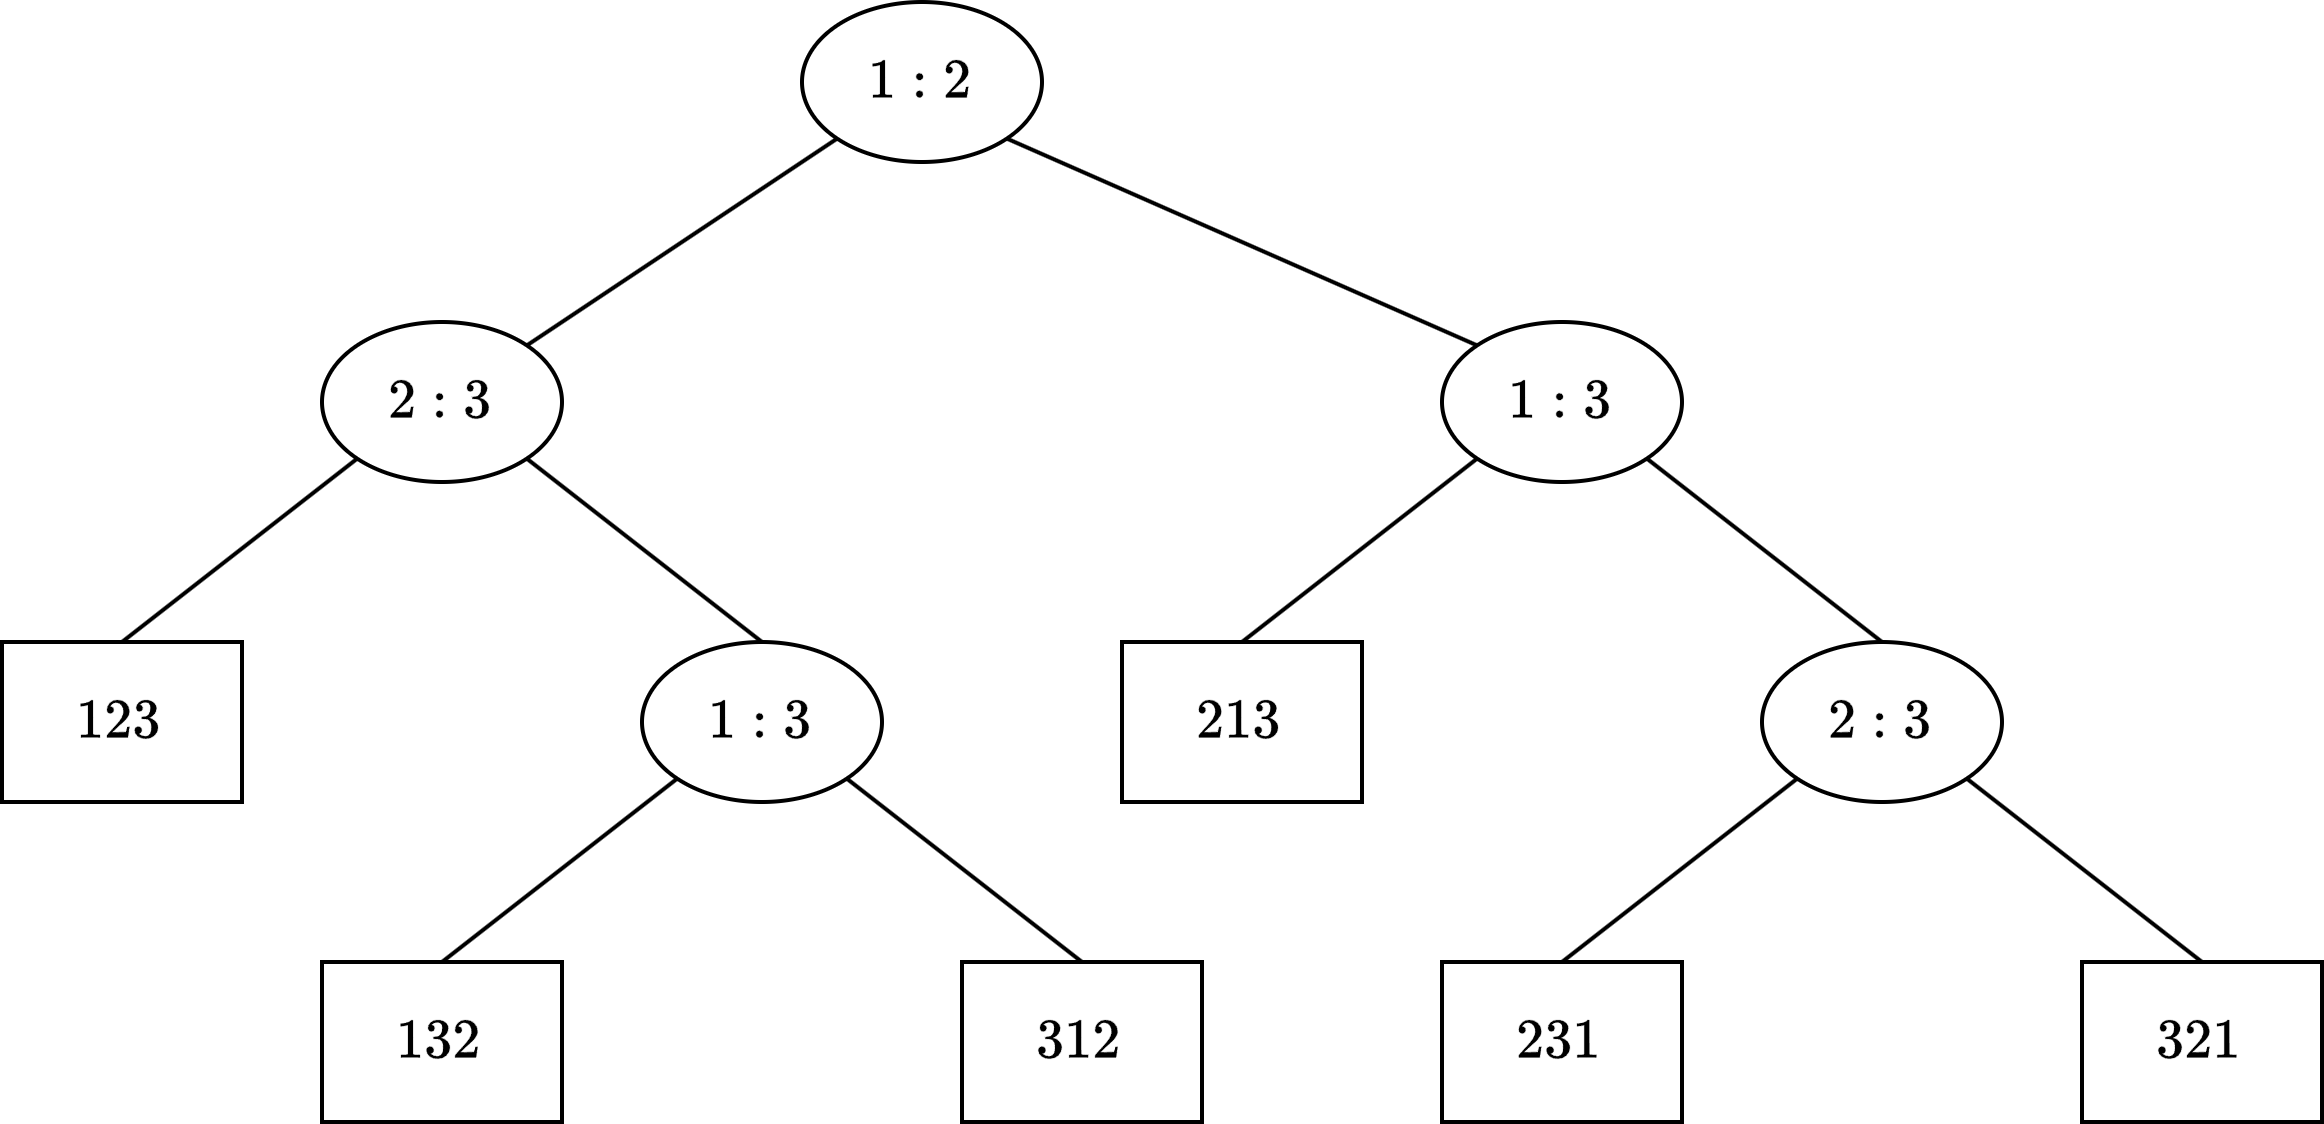
\includegraphics[width=0.8\linewidth]{images/tree1.png}
    \end{figure}
    This decision tree helps visualize the comparisons made to sort the array, with each path from the root to a leaf representing a specific sequence of comparisons.
\end{example}
Each leaf in the decision tree represents a permutation $\left\langle \pi (1), \pi (2),\dots, \pi (n)\right\rangle $, indicating the established sorted order $a_{\pi(1)}\leq a_{\pi(2)} \leq\dots\leq a_{\pi(n)}$.

The height of the decision tree corresponds to the worst-case running time of the algorithm, as it reflects the maximum number of comparisons made during the sorting process.
The worst-case running time is the length of the longest path from the root to a leaf node, which is the height of the tree.

Since there are $n!$ possible ways to order $n$ distinct elements, the decision tree must have at least $n!$ leaves. 
A binary tree of height $h$ has at most $2^h$ leaves.
Therefore, we must have $2^h\geq n!$.
Taking the logarithm on both sides:
\[h\geq \log n!\]
Applying Stirling's approximation $n!\approx\left(\frac{n}{e}\right)^n$, we have:
\[\log n!\geq n\log n-n\log e\]
Thus, the height of the decision tree (and hence the worst-case running time of any comparison sort) is at least:
\[h=\Omega(n\log n)\]
This proves that any comparison-based sorting algorithm must have a worst-case time complexity of $\Omega(n\log n)$, which is a lower bound for all comparison sorts.
\begin{theorem}
    Any decision tree that can sort n elements must have height $\Omega(n \log n)$.
\end{theorem}
\begin{corollary}
    Since heapsort and merg esort both achieve a worst-case time complexity of $\mathcal{O}(n\log n)$, they are asymptotically optimal comparison sorting algorithms.
\end{corollary}

\subsection{Counting sort}
Counting sort is a non-comparison-based sorting algorithm. 
It leverages the range of possible values in the input to efficiently organize the elements.

This algorithm takes as input an array $A[n]$, where each element $A[j]\in\{1, 2, \dots, k\}$, and returns a sorted array $B[n]$.
It also needs an auxiliary array $C[n]$. 
\begin{algorithm}[H]
    \caption{Counting sort}
    \begin{algorithmic}[1]
        \For{$i=1$ \textbf{ to } $k$} \Comment Set all elements of array $C$ to zero.
            \State $C[i]=0$ 
        \EndFor \Comment Complexity $\Theta(k)$
        \For{$j=1$ \textbf{ to } $n$} \Comment Count how many times each element appears in the input array $A$
            \State $C[A[j]]=C[A[j]]+1$ 
        \EndFor \Comment Complexity $\Theta(n)$
        \For{$i=2$ \textbf{ to } $k$} \Comment Compute the prefix sum for each element in $C$
            \State $C[i]=C[i]+C[i-1]$ 
        \EndFor \Comment Complexity $\Theta(k)$
        \For{$j=n$ \textbf{ to } $1$} \Comment Place elements into output array $B$ and reduce counters in $C$
            \State $B[C[A[j]]]=A[j]$
            \State $C[A[j]]=C[A[j]]-1$ 
        \EndFor \Comment Complexity $\Theta(n)$
    \end{algorithmic}
\end{algorithm}  
\begin{example}
    Let's consider an example where we sort the array $A=\left\langle 4, 1, 3, 4, 3\right\rangle$, with $k=4$. 
    \begin{enumerate}
        \item \textit{Initial state}: we initialize the array $C$ to all zeros: $C=\left\langle 0,0,0,0\right\rangle$.
        \item \textit{Count elements}: we count the occurrences of each element in $A$, resulting in: $C=\left\langle 1,0,2,2\right\rangle$.
        \item \textit{Compute the prefix sum}: we compute the prefix sum over $C$: $C=\left\langle 1,1,3,5\right\rangle$.
        \item \textit{Place elements into output array}: starting from the last element of $A$, we place elements into their correct position in $B$ using the cumulative counts in $C$, and decrement the counts as we go. 
            The final result will be: $B=\left\langle 1,3,3,4,4\right\rangle$ and $C=\left\langle 0,1,1,3\right\rangle$.
    \end{enumerate}
\end{example}
We have that the complexity of the algorithm is the sum of the complexities of the four loops: 
\[\Theta(k)+\Theta(n)+\Theta(k)+\Theta(n)\]
Thus, the total time complexity of counting sort is: 
\[\Theta(n+k)\]
If $k = \mathcal{O}(n)$, then counting sort runs in linear time, $\Theta(n)$.

\paragraph*{Stability}
Counting sort is a stable sort, meaning it preserves the relative order of equal elements from the input array. 
This stability can be particularly important in scenarios where sorting must maintain additional orderings or properties of the data.

\subsection{Radix sort}
Radix sort is a classic algorithm with historical significance, dating back to Herman Hollerith's card-sorting machine developed for the 1890 U.S. Census. 
The core concept of radix sort is to sort numbers digit by digit, which can be efficient for large inputs under certain conditions.

The original method proposed by Hollerith was to sort starting with the most significant digit first, but this approach turned out to be inefficient. 
Instead, the more effective strategy is to sort based on the least significant digit first, using an auxiliary stable sort like counting sort.

\paragraph*{Correctness}
To ensure correctness assume that the numbers have already been sorted by their least significant $t-1$ digits.
Now sort the numbers by the $t$-th digit: 
\begin{itemize}
    \item Two numbers that differ in the $t$-th digit will be correctly ordered.
    \item Two numbers that are identical in the $t$-th digit will retain their original relative order (thanks to the stability of the auxiliary sort).
\end{itemize}
This results in the numbers being in the correct final order.

\paragraph*{Performance analysis}
To analyze the efficiency of radix sort, assume we are using counting sort as the stable auxiliary sorting method. 
Suppose we are sorting $n$ computer words, each consisting of $b$ bits. 
Each word can be viewed as having $\frac{b}{r}$ digits, where each digit is based on $2^r$. 

The time complexity of each pass of counting sort is $\Theta(n + 2^r)$, since we process $n$ numbers and there are $2^r$ possible values for each digit.
The total number of passes is $\frac{b}{r}$, so the overall time complexity is given by:
\[T(n,b)=\Theta\left(\dfrac{b}{r}(n+2^r)\right)\]
To minimize the time complexity, we must choose an optimal $r$.
Increasing $r$ reduces the number of passes (since $\frac{b}{r}$ becomes smaller), but it also increases $2^r$, which can inflate the running time.
For efficiency, we should avoid letting $2^r$ become larger than $n$, as this leads to exponential growth in time.
Thus, an optimal choice is to set $r=\log n$, which balances the number of passes and the cost of each pass. 
With this choice, the time complexity becomes:
\[T(n,b)=\Theta\left(\dfrac{bn}{\log n}\right)\]
For numbers in the range from $0$ to $n^d-1$, where $b=d\log n$, the radix sort runs in $\Theta(dn)$ time. 

In practice, radix sort is particularly fast for large datasets and is simple to implement. 
However, it exhibits poor locality of reference compared to algorithms like quicksort, which can cause performance issues on modern processors with complex memory hierarchies. 
As a result, a well-optimized quicksort may outperform radix sort in environments where memory access speed is crucial.